\section{Modello finale}
In fase di modellazione sono state modificate le quote del lamone-piastrone per permettere l'accoppiamento con le carrucole e la traversa. 
La distanza tra il foro per l'asse della traversa e quello dell'asse delle carrucole risultavano infatti troppo vicini, il carter superiore andava poi a compenetrare le carrucole. 
Lo spessore di lamoni e piastroni è risultato essere adeguato, non sono state apportate modifiche rispetto alla fase di progettazione nominale.
Sono state modificate le quote della traversa in quanto gli sforzi che si instaurano sulla parte inferiore del raccordo del perno sono elevati. 
Per mantenere adeguato il coefficiente di sicurezza, si è scelto di usare un acciaio legato con migliori prestazioni le cui proprietà sono mostrate in tabella \ref{tab:PropLega}. 
\begin{table}[H]
\centering
\begin{tabular}{lc}
\toprule
Modulo elastico         & $210 \; GPa$    \\
Coeff. di Poisson       & $0.28$      \\
Modulo di taglio        & $79 \; GPa$     \\
Densità                 & $7700 \; kg/m^3$ \\
Resistenza a trazione   & $723.8 \; MPa$  \\
Tensione di snervamento & $620.4 \; MPa$ \\
\bottomrule
\end{tabular}
\caption{Proprietà acciaio legato.}
\label{tab:PropLega}
\end{table} 
Per gli altri componenti è stato utilizzato un AISI 1020.
\begin{table}[H]
\centering
\begin{tabular}{lc}
\toprule
Modulo elastico         & $200 \; GPa$    \\
Coeff. di Poisson       & $0.29$      \\
Modulo di taglio        & $77 \; GPa$     \\
Densità                 & $7700 \; kg/m^3$ \\
Resistenza a trazione   & $420.5 \; MPa$  \\
Tensione di snervamento & $351.5 \; MPa$ \\
\bottomrule
\end{tabular}
\caption{Proprietà AISI 1020.}
\label{tab:aisi1020}
\end{table} 
Per la movimentazione del gancio è stato inserito un golfare machio\footnote{Fare riferimento al catalogo presente in appendice} M30 sul rinforzo superiore; è risultato necessario incrementare lo spessore dello stesso fino ad un valore pari alla lunghezza della filettatura del golfare.
In appendice è presente il catalogo dei golfari. Si è optato per un M30, in questo modo si garantisce la tenuta anche per movimentazioni che implicano una sollecitazione del golfare a $90^{\circ}$ rispetto al proprio asse ($portata di 1600 \; kg$). 
Le masse dei componenti sono riportate in tabella, la bulloneria non è stata considerata in quanto avente un contributo irrisorio.
\begin{table}[]
\centering
\begin{tabular}{lc}
\toprule
                  & \begin{tabular}[c]{@{}c@{}}\textbf{Massa}\\ $[Kg]$\end{tabular} \\
                  \midrule
Puleggia          & $88.3$                                                 \\
Traversa con dado & $141.0$                                                \\
Lamone piastrone  & $701.6$                                                \\
Asse              & $78.9$                                                 \\
Gancio            & $264.0$                  \\ \hline
Massa totale      & $1273.8$ \\
\bottomrule                             
\end{tabular}
\caption{}
\label{tab:massaGancio}
\end{table}
L'ingrandimento mostra la presenza di una luce di scolo dell'acqua piovana e i tiranti di irrigidimento. 
\begin{figure}[h!]
\centering
  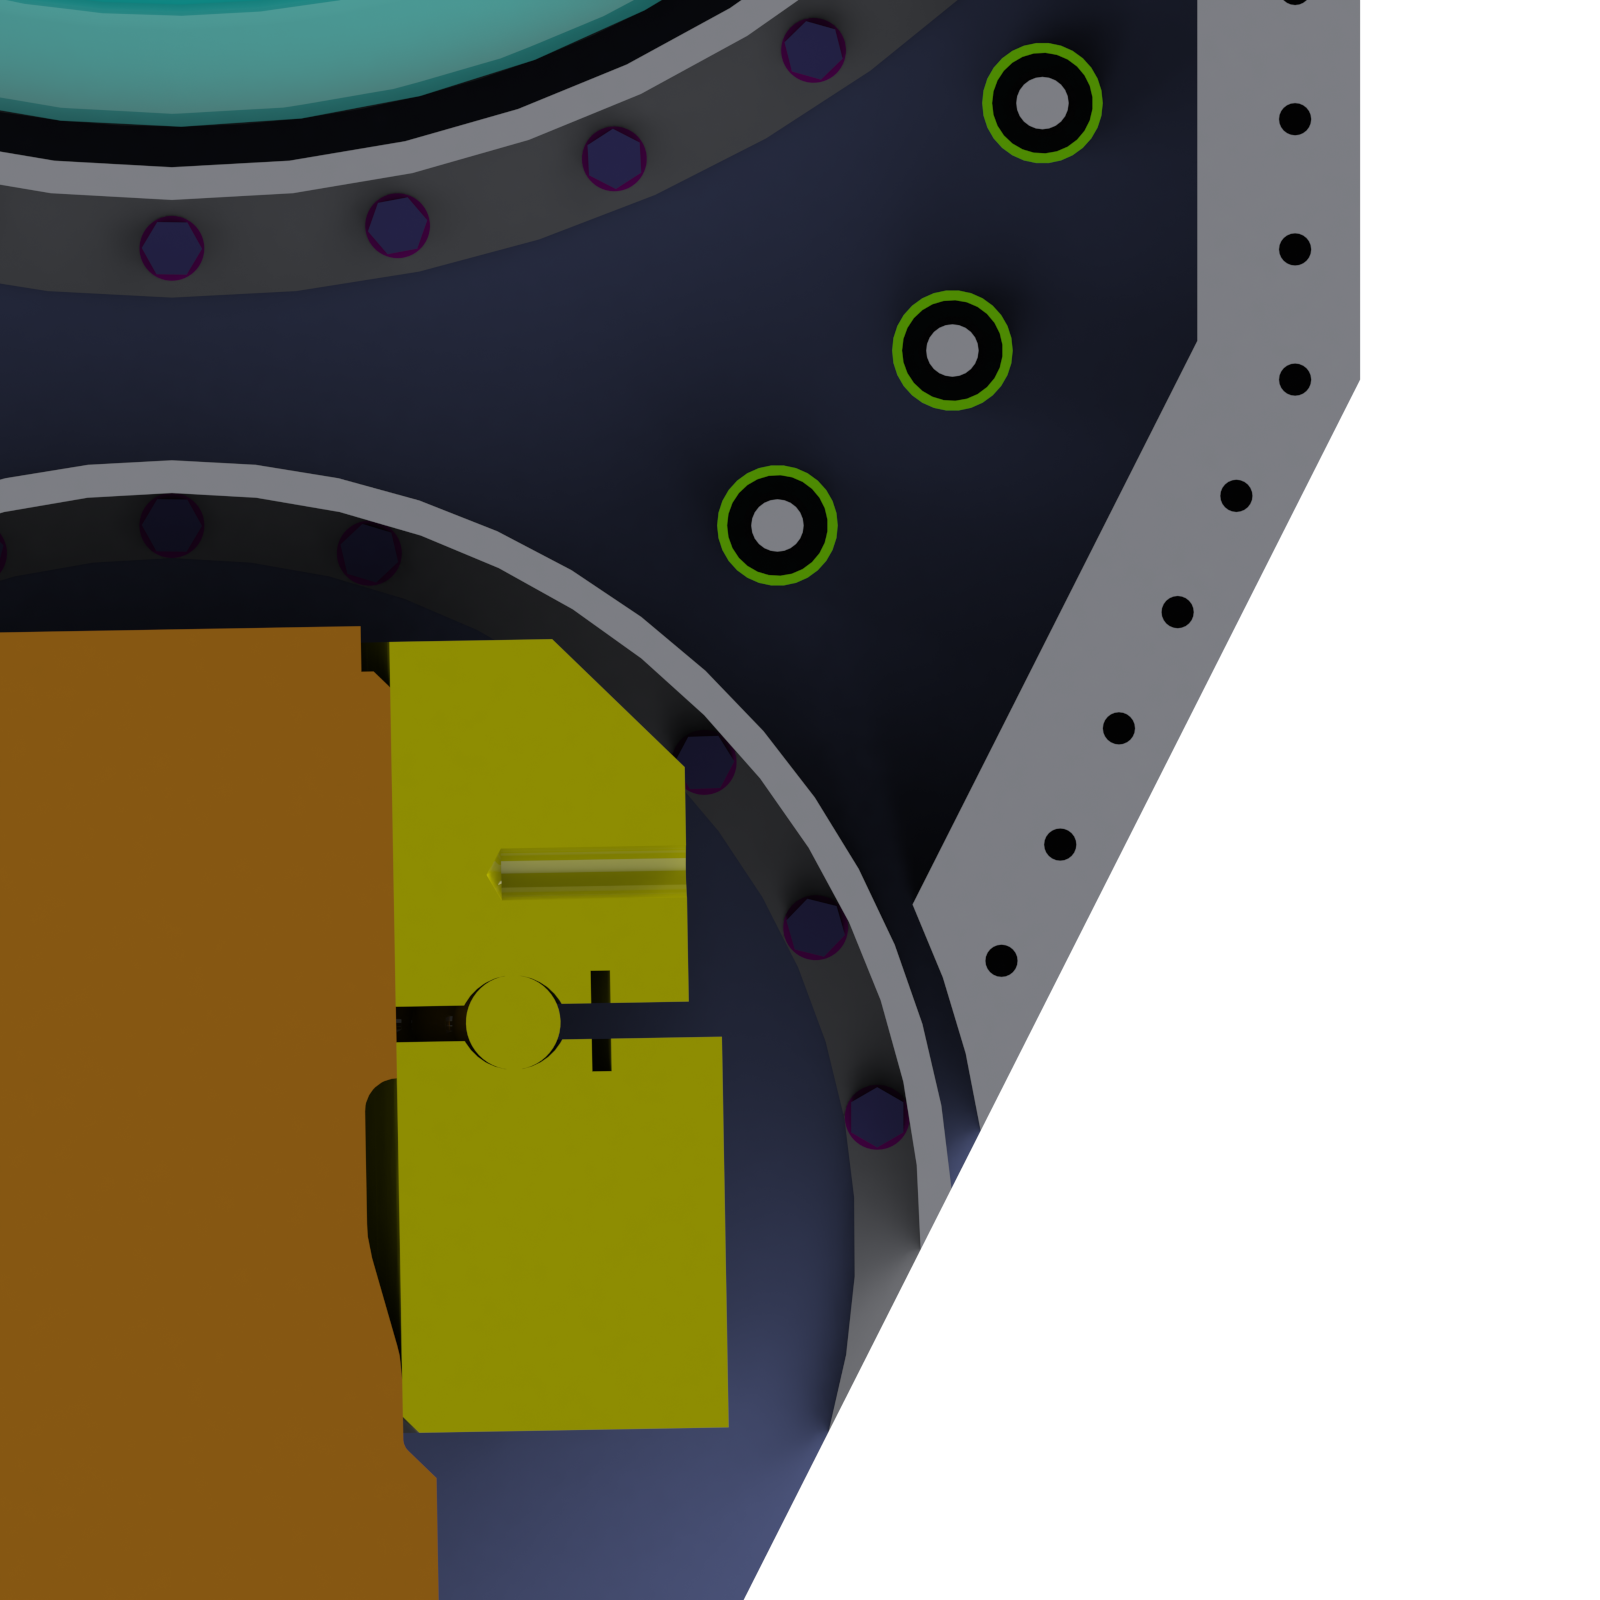
\includegraphics[width=.4\textwidth]{render/Dettaglio}
\caption{}
\label{fig:Dettaglio}
\end{figure}
\begin{figure}[h!]
\centering
  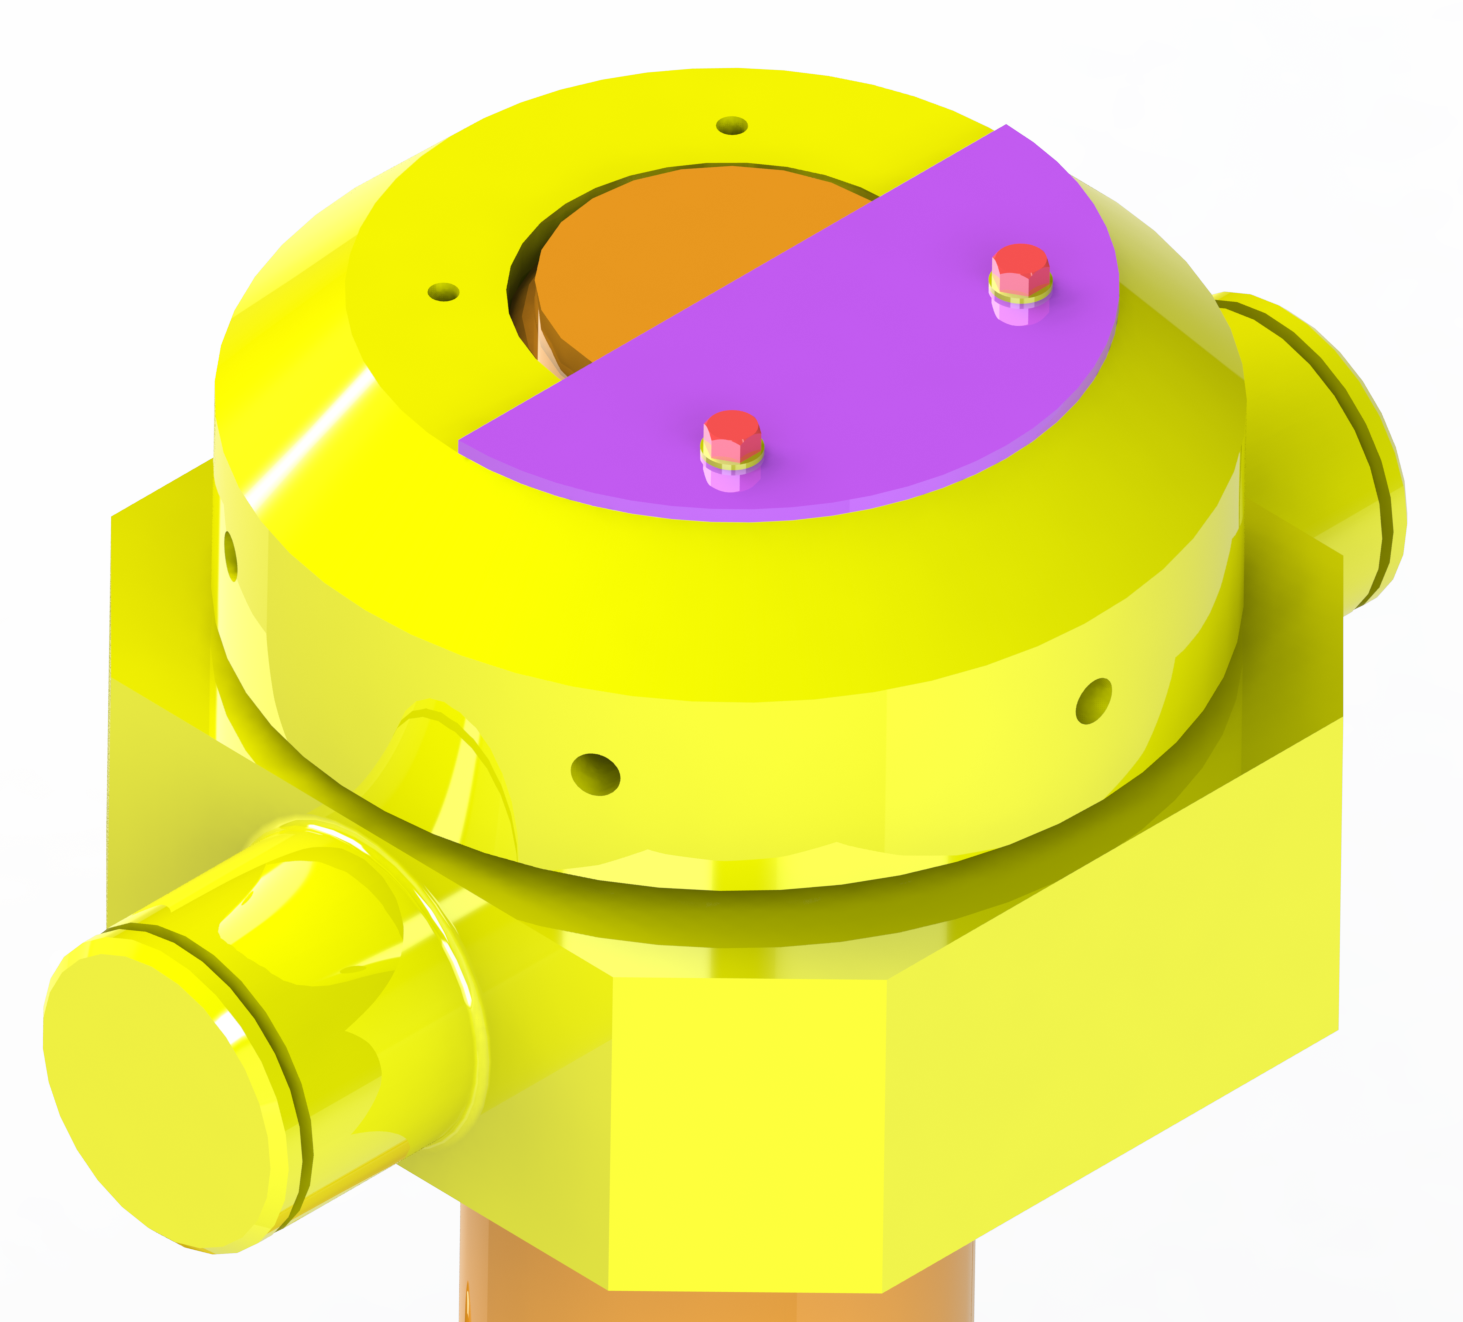
\includegraphics[width=.4\textwidth]{render/PiastrinaGancio}
\caption{}
\label{fig:PiastrinaGancio}
\end{figure}
In figura \ref{fig:Gancio1} è possibile vedere il modello finale. 
\begin{figure}[h!]
\centering
  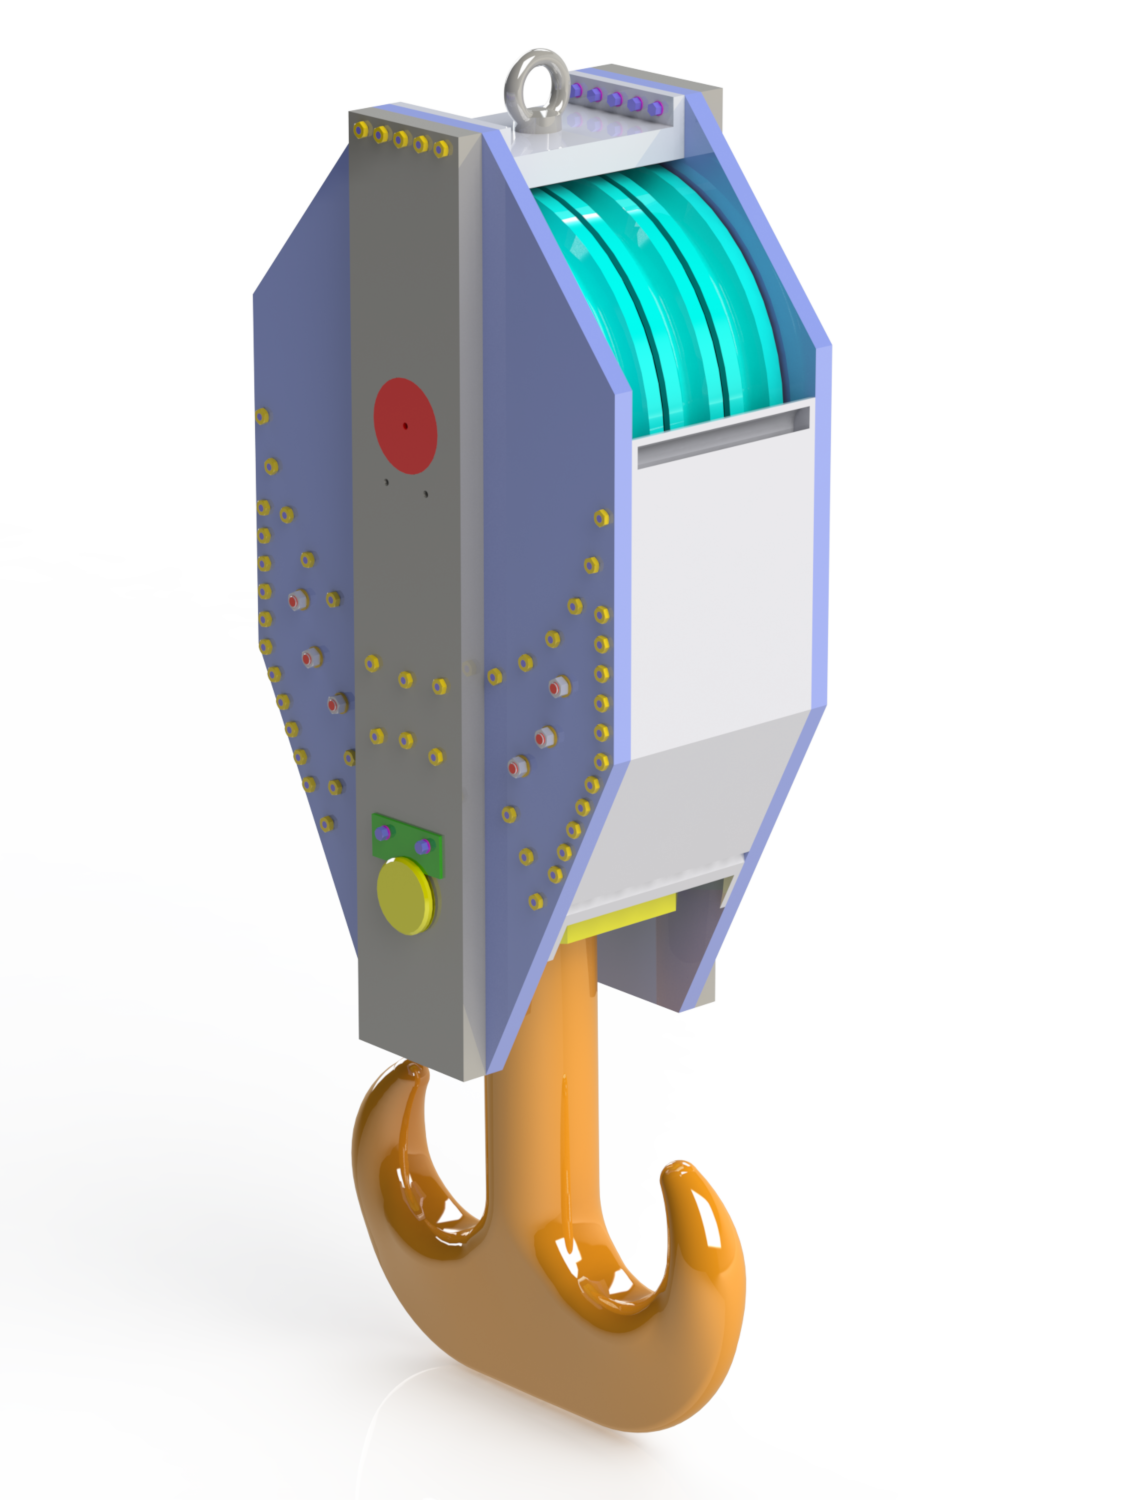
\includegraphics[width=.6\textwidth]{render/Gancio1}
\caption{}
\label{fig:Gancio1}
\end{figure}
Di seguito viene mostrata una sezione di metà bozzello.
\begin{figure}[h!]
\centering
  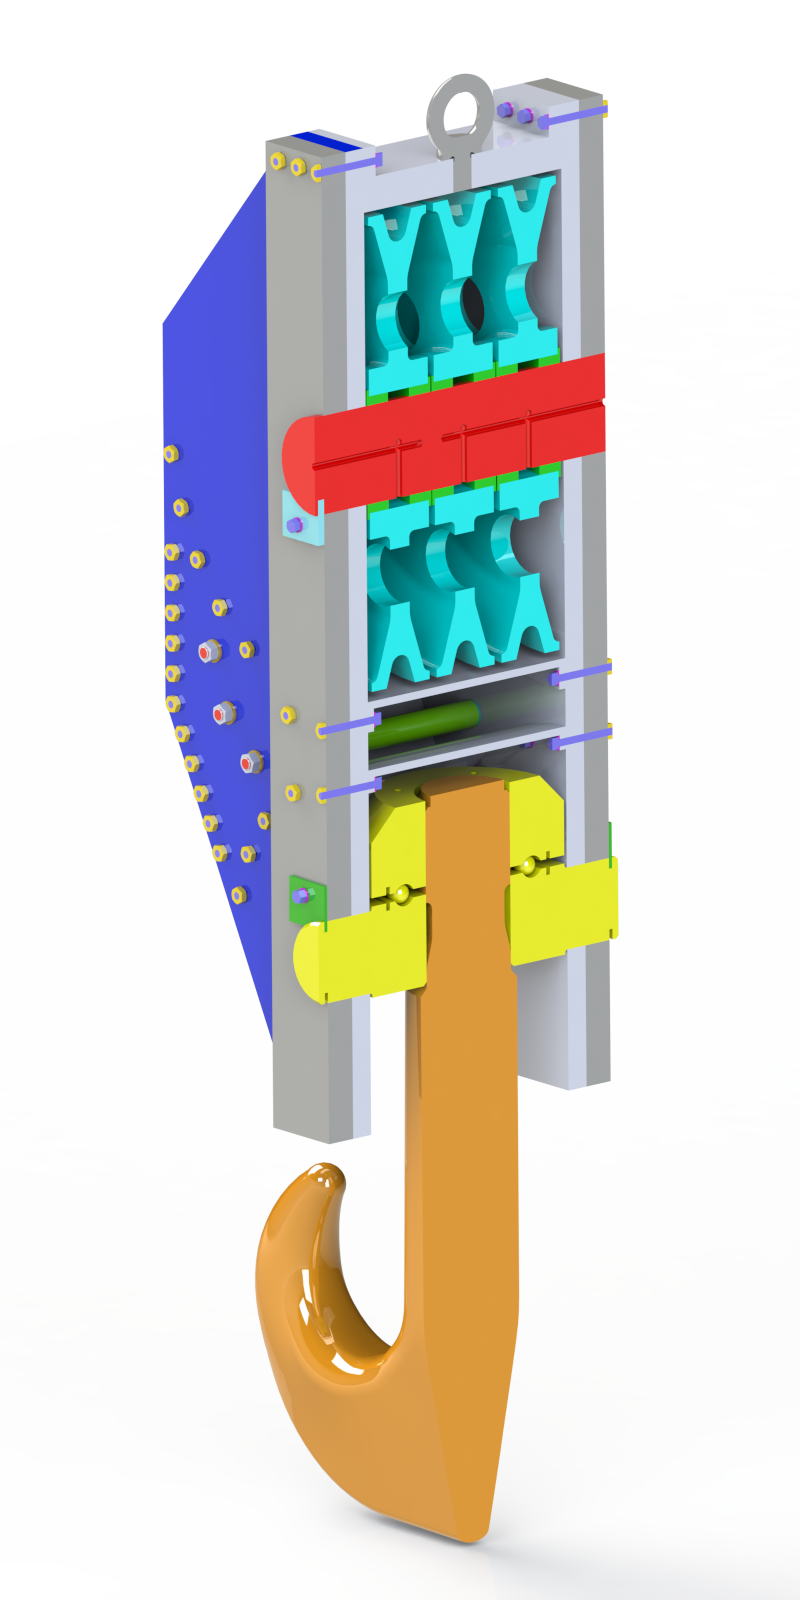
\includegraphics[width=.4\textwidth]{render/GancioSezione}
\caption{}
\label{fig:GancioSezione}
\end{figure}
